% !TEX program = lualatex
\documentclass[aspectratio=43,professionalfonts,handout]{beamer}
\usepackage{beamer_template}

\newcommand{\LectureNum}{02}
\newcommand{\LectureTitle}{２次関数のグラフ（１）}
\newcommand{\TextPages}{p.\,75-77}
\newcommand{\NextTopic}{２次関数のグラフ（２）}
\newcommand{\NextPages}{p.\,77-79}
\newcommand{\CourseName}{基礎数学B}
\renewcommand{\TermName}{前期}

\begin{document}

% -----------------------------------------------
% スライド1: 表紙＋目標＋用語・定義
% -----------------------------------------------
\begin{frame}{\CourseName\quad 第\LectureNum 回「\LectureTitle 」}
  {\small \TermName\quad \TeacherName\quad ／\quad 教科書 \TextPages\quad
  \textbf{目標}：y=ax²のグラフと平行移動を理解し、標準形に変形できる}

  \begin{block}{用語・定義}
  \begin{description}[labelwidth=5.5em]
    \item[\kw{2次関数}] ~
    \item[\kw{放物線}] ~
    \item[\kw{軸}] ~
    \item[\kw{頂点}] ~
    \item[\kw{標準形}] ~
  \end{description}
  \end{block}
\end{frame}

% -----------------------------------------------
% スライド2: 公式・性質
% -----------------------------------------------
\begin{frame}{公式・性質}
  \begin{block}{}
  \begin{itemize}
    \item y=ax² のグラフの性質
    \item 平行移動の規則 y=a(x-p)²+q
  \end{itemize}
  \end{block}
\end{frame}

% -----------------------------------------------
% スライド3: 図・グラフ（TikZコードを手動追加）
% -----------------------------------------------
\begin{frame}{図・グラフ}
  \centering
  % TODO: y=x²、y=(x-2)²、y=(x-2)²+3 の比較
  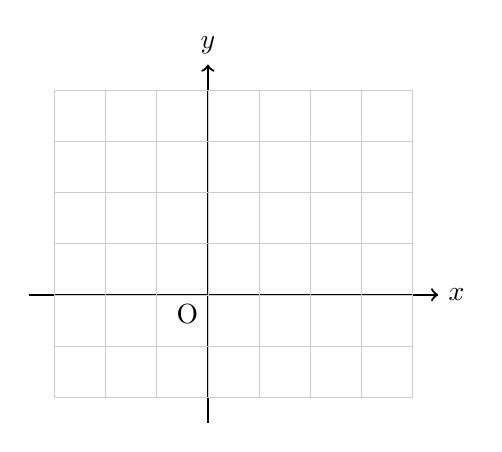
\begin{tikzpicture}[scale=0.65]
    \draw[->,thick] (-3.5,0) -- (4.5,0) node[right]{$x$};
    \draw[->,thick] (0,-2.5) -- (0,4.5) node[above]{$y$};
    \node[below left] at (0,0) {O};
    \draw[gray!40, very thin] (-3,-2) grid (4,4);
    % ここにグラフを描画
  \end{tikzpicture}
\end{frame}

% -----------------------------------------------
% スライド4: 例1→問1
% -----------------------------------------------
\begin{frame}{例1→問1}
  \begin{exampleblock}{例4) p.76（軸・頂点）}
    （板書で解説）
  \end{exampleblock}

  \vfill

  \begin{block}{問3) p.76（グラフをかけ）\quad 自分で解いてみよう}
    （ノートに解くこと）
  \end{block}
\end{frame}

% -----------------------------------------------
% スライド5: 例2→問2
% -----------------------------------------------
\begin{frame}{例2→問2}
  \begin{exampleblock}{例4) p.76（平行移動の方程式）}
    （板書で解説）
  \end{exampleblock}

  \vfill

  \begin{block}{問4) p.76\quad 自分で解いてみよう}
    （ノートに解くこと）
  \end{block}
\end{frame}

% -----------------------------------------------
% まとめ
% -----------------------------------------------
\begin{frame}{まとめ}
  \begin{itemize}
    \item y=a(x-p)²+q が標準形：軸 x=p、頂点 (p,q)
    \item a>0 で下に凸、a<0 で上に凸
    \item x 軸方向に p 平行移動 → x を x-p に置き換える
    \item y 軸方向に q 平行移動 → 右辺に +q
  \end{itemize}

  \vfill
  {\small 基本問題：145, 146}
\end{frame}

\end{document}
